\documentclass{article}
\usepackage[paperwidth=11in,paperheight=8.5in,margin=0.28in]{geometry}
\usepackage[T1]{fontenc}
\usepackage{tikz}
\usetikzlibrary{arrows.meta,positioning,fit,calc,shapes.geometric}
\pagestyle{empty}

\begin{document}
\begin{center}
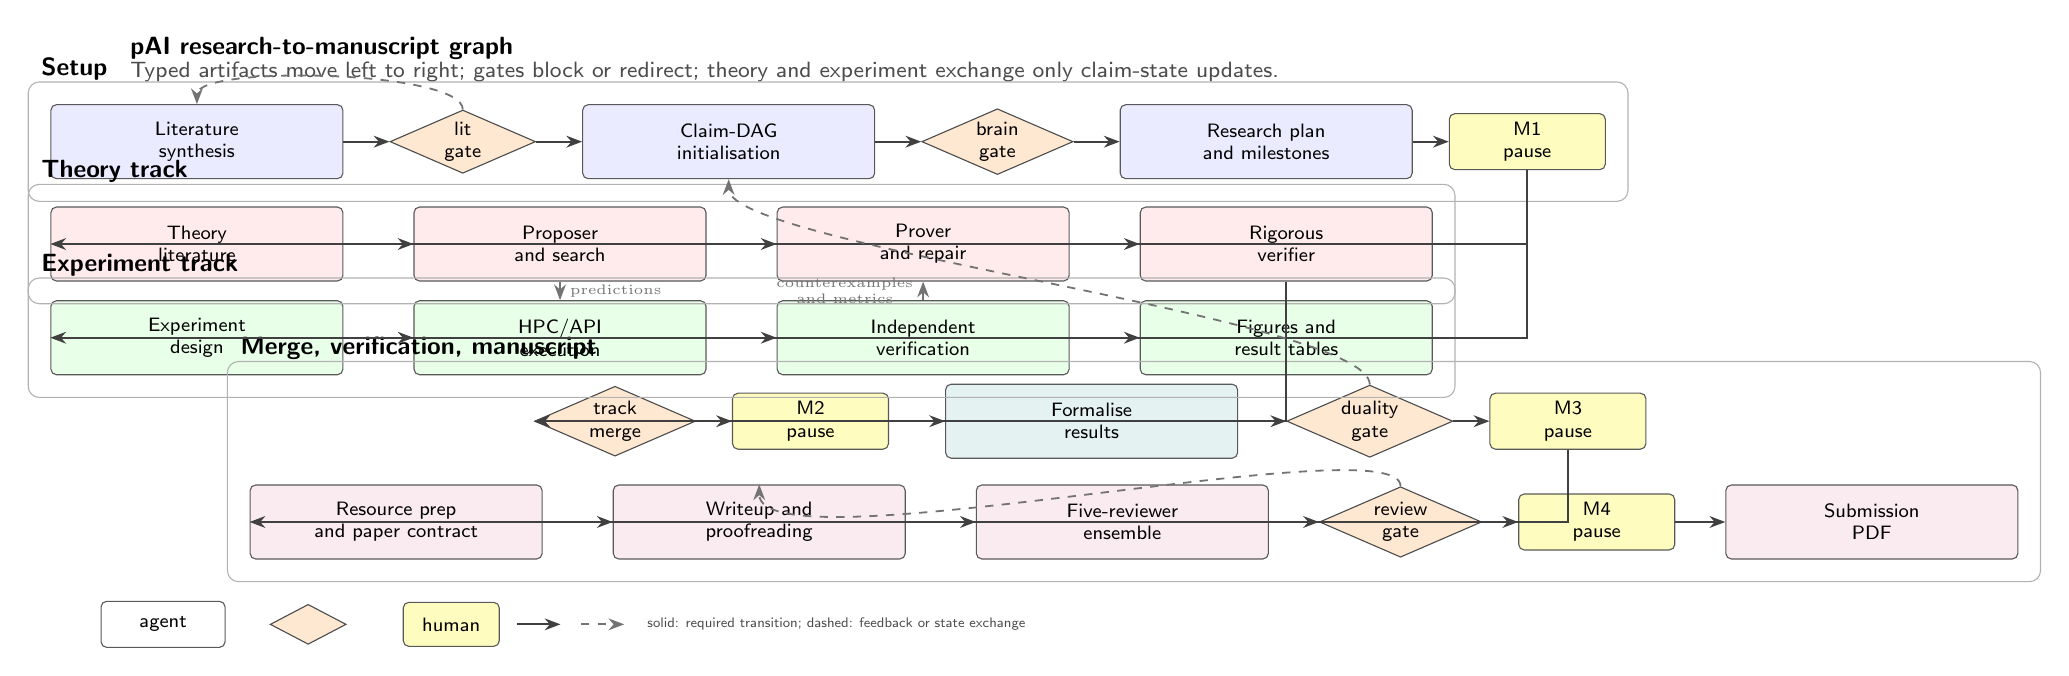
\begin{tikzpicture}[
  font=\sffamily\scriptsize,
  >={Stealth[length=2.0mm]},
  stage/.style={rectangle,rounded corners=2pt,draw=black!65,fill=white,
    minimum width=1.46in,minimum height=0.37in,align=center,inner sep=3pt},
  gate/.style={diamond,aspect=2.3,draw=black!70,fill=orange!18,
    minimum width=0.62in,minimum height=0.30in,align=center,inner sep=1pt},
  human/.style={rectangle,rounded corners=2pt,draw=black!65,fill=yellow!25,
    minimum width=0.78in,minimum height=0.28in,align=center,inner sep=2pt},
  lane/.style={rectangle,rounded corners=4pt,draw=black!30,inner sep=8pt},
  arr/.style={->,line width=0.7pt,black!75},
  soft/.style={->,line width=0.65pt,dashed,black!55},
  label/.style={font=\sffamily\bfseries\small,anchor=west}
]

\node[label] at (-5.12,3.74) {pAI research-to-manuscript graph};
\node[font=\sffamily\footnotesize,anchor=west,text=black!70] at (-5.12,3.43)
  {Typed artifacts move left to right; gates block or redirect; theory and experiment exchange only claim-state updates.};

% Setup lane
\node[stage,fill=blue!8] (lit) at (-4.15,2.55) {Literature\\synthesis};
\node[gate] (litg) [right=0.23in of lit] {lit\\gate};
\node[stage,fill=blue!8] (brain) [right=0.23in of litg] {Claim-DAG\\initialisation};
\node[gate] (braing) [right=0.23in of brain] {brain\\gate};
\node[stage,fill=blue!8] (plan) [right=0.23in of braing] {Research plan\\and milestones};
\node[human] (m1) [right=0.18in of plan] {M1\\pause};

% Theory lane
\node[stage,fill=red!8] (t1) at (-4.15,1.25) {Theory\\literature};
\node[stage,fill=red!8] (t2) [right=0.35in of t1] {Proposer\\and search};
\node[stage,fill=red!8] (t3) [right=0.35in of t2] {Prover\\and repair};
\node[stage,fill=red!8] (t4) [right=0.35in of t3] {Rigorous\\verifier};

% Experiment lane
\node[stage,fill=green!9] (e1) at (-4.15,0.06) {Experiment\\design};
\node[stage,fill=green!9] (e2) [right=0.35in of e1] {HPC/API\\execution};
\node[stage,fill=green!9] (e3) [right=0.35in of e2] {Independent\\verification};
\node[stage,fill=green!9] (e4) [right=0.35in of e3] {Figures and\\result tables};

% Merge and manuscript lane
\node[gate] (merge) at (1.16,-1.00) {track\\merge};
\node[human] (m2) [right=0.18in of merge] {M2\\pause};
\node[stage,fill=teal!10] (formal) [right=0.28in of m2] {Formalise\\results};
\node[gate] (duality) [right=0.24in of formal] {duality\\gate};
\node[human] (m3) [right=0.18in of duality] {M3\\pause};
\node[stage,fill=purple!8] (write) at (-1.62,-2.28) {Resource prep\\and paper contract};
\node[stage,fill=purple!8] (draft) [right=0.35in of write] {Writeup and\\proofreading};
\node[stage,fill=purple!8] (review) [right=0.35in of draft] {Five-reviewer\\ensemble};
\node[gate] (finalg) [right=0.25in of review] {review\\gate};
\node[human] (m4) [right=0.18in of finalg] {M4\\pause};
\node[stage,fill=purple!8] (pdf) [right=0.25in of m4] {Submission\\PDF};

% Lane boxes and labels
\node[lane,fit=(lit)(litg)(brain)(braing)(plan)(m1)] (setupbox) {};
\node[lane,fit=(t1)(t2)(t3)(t4)] (theorybox) {};
\node[lane,fit=(e1)(e2)(e3)(e4)] (expbox) {};
\node[lane,fit=(merge)(m2)(formal)(duality)(m3)(write)(draft)(review)(finalg)(m4)(pdf)] (paperbox) {};
\node[label] at ($(setupbox.north west)+(0.05,0.16)$) {Setup};
\node[label] at ($(theorybox.north west)+(0.05,0.16)$) {Theory track};
\node[label] at ($(expbox.north west)+(0.05,0.16)$) {Experiment track};
\node[label] at ($(paperbox.north west)+(0.05,0.16)$) {Merge, verification, manuscript};

% Arrows setup
\draw[arr] (lit) -- (litg);
\draw[arr] (litg) -- (brain);
\draw[arr] (brain) -- (braing);
\draw[arr] (braing) -- (plan);
\draw[arr] (plan) -- (m1);
\draw[arr] (m1.south) |- (t1.west);
\draw[arr] (m1.south) |- (e1.west);

% Arrows tracks
\draw[arr] (t1) -- (t2);
\draw[arr] (t2) -- (t3);
\draw[arr] (t3) -- (t4);
\draw[arr] (e1) -- (e2);
\draw[arr] (e2) -- (e3);
\draw[arr] (e3) -- (e4);
\draw[soft] (t2.south) -- node[right,font=\tiny,align=center] {predictions} (e2.north);
\draw[soft] (e3.north) -- node[left,font=\tiny,align=center] {counterexamples\\and metrics} (t3.south);

% Merge and manuscript
\draw[arr] (t4.south) |- (merge.west);
\draw[arr] (e4.south) |- (merge.west);
\draw[arr] (merge) -- (m2);
\draw[arr] (m2) -- (formal);
\draw[arr] (formal) -- (duality);
\draw[arr] (duality) -- (m3);
\draw[arr] (m3.south) |- (write.west);
\draw[arr] (write) -- (draft);
\draw[arr] (draft) -- (review);
\draw[arr] (review) -- (finalg);
\draw[arr] (finalg) -- (m4);
\draw[arr] (m4) -- (pdf);

% Feedback routes
\draw[soft] (duality.north) .. controls +(0,0.85) and +(0,-0.85) .. (brain.south);
\draw[soft] (finalg.north) .. controls +(0,0.80) and +(0,-1.10) .. (draft.north);
\draw[soft] (litg.north) .. controls +(0,0.50) and +(0,0.50) .. (lit.north);

% Legend
\node[stage,minimum width=0.62in,minimum height=0.23in,fill=white] (la) at (-4.58,-3.58) {agent};
\node[gate,minimum width=0.38in,minimum height=0.20in] (lg) [right=0.22in of la] {};
\node[human,minimum width=0.48in,minimum height=0.22in] (lh) [right=0.28in of lg] {human};
\draw[arr] ($(lh.east)+(0.22,0)$) -- +(0.55,0);
\draw[soft] ($(lh.east)+(1.03,0)$) -- +(0.55,0);
\node[anchor=west,font=\sffamily\tiny,text=black!70] at ($(lh.east)+(1.75,0)$)
 {solid: required transition; dashed: feedback or state exchange};

\end{tikzpicture}
\end{center}
\end{document}
